\documentclass{beamer}
\usetheme{Madrid}
\usecolortheme{default}

% Packages
\usepackage{graphicx}
\usepackage{amsmath}
\usepackage{tikz}
\usetikzlibrary{shapes.geometric, arrows, positioning}

% Title Page
\title{A Generalized Vehicle Routing Problem Optimization based on Gavish and Graves Formulation (1978)}

\author{Christos - Chrysovalantis Paraschakis \and Dimitrios Charistes}
\institute{University of Western Macedonia - \\
Department of Electrical and Computer Engineering}

\date{\today}

\begin{document}

% Title Slide
\begin{frame}
    \titlepage
\end{frame}

% Outline
\begin{frame}{Outline}
    \tableofcontents
\end{frame}

% Introduction
\begin{frame}{Introduction}
    \small % Adjust font size for better fit
    
    \begin{itemize}
        \item The GVR problem that was modeled is the Ganish and Graves (1976) formulation.
        \item The goal of the GVRP is to minimize total traversal costs across the set of arcs $A$ by servicing all cluster demands using exactly one node within it.
    \end{itemize}
    
    \vspace{-0.5em} % Reduce spacing for compactness
    
    % \textbf{Mathematical Formulation of SCP:}
    \[
    \min \sum_{(i,j) \in A} c_{ij}x_{ij}
    \]

    where:
    \begin{itemize}
        \item \( A \) is the set of all arcs in the directed Graph $G(V,A)$.
        \item \( c_{ij} \) is the cost of the arc $(i,j)$ 
        \item \( x_{ij}\in \{0,1\} \) is the arc $(i,j)$. If the arc is used it is 1.
    \end{itemize}
\end{frame}

% Problem Formulation
\section{Problem Formulation}
\begin{frame}{Problem Formulation}
    \begin{itemize}
        \item Modeled as an MILP with the arc variable being a integer and the flow variable by implication is integer although it is modeled as continuous.
        \item Constraints: \begin{itemize}
            \item Cluster Visit Rule
            \item Vehicle Usage Rule
            \item Flow Conservation Rule
            \item Commodity Flow Balance
            \item Capacity Constraint
        \end{itemize}
        \item Objective: \textbf{Minimize travel cost.}
    \end{itemize}

\end{frame}




% ILP Model Slide
\begin{frame}{GVRP Mathematical Formulation}
    % 1. Use footnotesize to save space
    \footnotesize 
    
    % 2. Tighten math spacing globally for this slide
    \setlength{\abovedisplayskip}{3pt}
    \setlength{\belowdisplayskip}{3pt}

    \textbf{Objective Function:}
    \[
    \text{Minimize} \quad \sum_{(i,j)\in A} c_{ij}x_{ij}
    \]
    
    \textbf{Subject to:}
    \begin{itemize}
        \setlength{\itemsep}{0pt}
        
        \item \textbf{Cluster Visit Rule:}
        \[
        x(\delta^+(C_k)) = 1, \quad x(\delta^-(C_k)) = 1 \quad \forall k \in M \setminus \{0\}
        \]
        
        \item \textbf{Vehicle \& Flow Conservation:}
        \[
        x(\delta^+(C_0)) = K, \quad x(\delta^-(C_0)) = K
        \]
        \[
        x(\delta^+(i)) = x(\delta^-(i)) \quad \forall i \in V
        \]
        
        \item \textbf{Commodity Flow Balance:}
        \[
        f(\delta^+(i)) - f(\delta^-(i)) = \frac{1}{2} q_{\alpha(i)}(x(\delta^-(i)) + x(\delta^+(i)))
        \]
        
        \item \textbf{Capacity \& Domain Constraints:}
        \[
        q_{\alpha(i)} \le f_{ij} \le (Q - q_{\alpha(i)})x_{ij} \quad \forall (i,j) \in A
        \]
        \[
        x_{ij} \in \{0, 1\} \quad \forall (i,j) \in A.
        \]
    \end{itemize}
\end{frame}

\begin{frame}{Using Gurobi as a Solver}
    \begin{itemize}
        \footnotesize
        \setlength{\itemsep}{1.0em} 
        
        \item \textbf{1. Instance Generation (\texttt{gvrppgenerator})}
        \begin{itemize}
            \item We create randomized problem instances using our custom generator.
            \item \textbf{Inputs:} Grid size ($N \times N$),Total number of Vertices ($V$),Number of Clusters, Vehicles ($K$), Capacity ($Q$), and the number of problems.
            \item \textbf{Output:} A .txt file containing all the information needed about the custom problem.
        \end{itemize}

        \item \textbf{2. Model Construction \& Execution}
        \begin{itemize}
            \item The generated data is loaded into \textbf{Gurobi}, and the SCF constraints (Equations 1-9) are initialized.
            \item The standard \texttt{model.optimize()} function is called, triggering Gurobi's internal \textbf{Branch-and-Cut} algorithm to find the best solution.
        \end{itemize}

        \item \textbf{3. Solution Extraction}
        \begin{itemize}
            \item We extract the active arcs ($x_{ij}=1$) to reconstruct the optimal route. 
        \end{itemize}
    \end{itemize}
\end{frame}

% Proposed Methodology
\section{Proposed Methodology}
\begin{frame}{Branch-and-Bound Method}
The Proposed methodology is based on a Branch and Cut algorithm. The problem is remodeled as LP in GurobiPy API. It will be compared to the PyOmo model.
    \begin{itemize}
        \item Utilizes \textbf{Best-First Search} technique.
        \item The nodes are inserted into a min-heap based on the relaxed objective solution.
        \item The most fractional variable of the node is explored first (Most-Fractional technique) $\rightarrow min_{i \in Ov}(value_i-0.5)$
        \item A Cutting Plane method is implemented inside this algorithm.
    \end{itemize}
\end{frame}

\begin{frame}{Heuristics}
    \begin{itemize}
        \item Heuristics are implemented to speed up the branching algorithm
        \item First, a Myopic Heuristic to extract an initial cost
        \item Then a metaheuristic VNS to improve the initial
        \item VNS's cost becomes the upper bound of the BnC 
    \end{itemize}
    \resizebox{\textwidth}{!}{%
    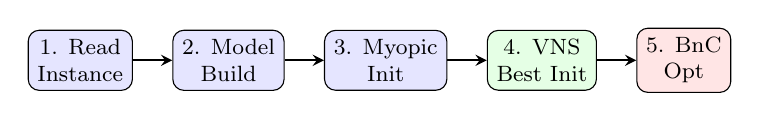
\begin{tikzpicture}[node distance=0.5cm, auto,
        process/.style={rectangle, draw=black, fill=blue!10, rounded corners, font=\footnotesize, align=center},
        arrow/.style={->, >=stealth, thick}]
    
        \node (input) [process] {1. Read\\Instance};
        \node (model) [process, right=of input] {2. Model\\Build};
        \node (myopic) [process, right=of model] {3. Myopic\\Init};
        \node (vns) [process, right=of myopic, fill=green!10] {4. VNS\\Best Init};
        \node (bnc) [process, right=of vns, fill=red!10] {5. BnC\\Opt};
    
        \draw [arrow] (input) -- (model);
        \draw [arrow] (model) -- (myopic);
        \draw [arrow] (myopic) -- (vns);
        \draw [arrow] (vns) -- (bnc);
    \end{tikzpicture}
}
\end{frame}

\begin{frame}{Variable Neighborhood Heuristic}
    \begin{itemize}
        \item Parameters $k_{max}$ and max\_iterations are set.
        \item Finds routes through the process: \begin{itemize}
            \item Shaking then local search
            \item Increases the intensity of shaking (if no improvement)
            \item The heuristic moves to the improved solution S'' only if feasibility criteria are checked.
        \end{itemize}
    \end{itemize}

    \begin{equation}
        (S, k) \leftarrow 
        \begin{cases} 
        (S'', 1) & \text{if } C(S'') < C(S) - \epsilon \\
        (S, k + 1) & \text{otherwise}
        \end{cases}
    \end{equation}
\end{frame}

\begin{frame}{Capacity Cut}
   \begin{itemize}
       \item The cut implemented in this algorithm is the \textit{Rounded Capacity Inequality}
       \item The cut enforces that at least $2r(S)$ arcs must cross the subset's boundary (accounting for both entry and exit).
   \end{itemize} 
   \begin{equation}
    r(S) = \left\lceil \frac{\sum_{k \in S} q_k}{Q} \right\rceil \le \frac{1}{2}\sum_{(i, j) \in \delta(S)} x_{ij}
    \end{equation}
   where:
   \begin{itemize}
       \item $S$ is a subset 
       \item $D(S)$ its total demand
       \item and $r(S)$ min vehicles required
   \end{itemize}

\end{frame}

% Results and Analysis
\section{Results and Analysis}
\begin{frame}{Experimental Setup}
    \begin{itemize}
        \item VNS parameters: $k_{max}=4 \;and\; max_{it}=100$.
        \item 5 problems with grid dimensions: \{10, 12, 14, 15, 35, 45\} generated.
        \item All Problems are solved by the BnC (final), BnB (simple) and Gurobi.
    \end{itemize}
\end{frame}

\begin{frame}{Performance Metrics}
    \begin{itemize}
        \item Key Metric 1: \textbf{Computation Time}.
        \item Key Metric 2: \textbf{Nodes Explored}
        \item Comparison between: \begin{itemize}
            \item ILP Model (Gurobi)
            \item Custom Branch and Cut Method
            \item Simple Branch and Bound
        \end{itemize}
    \end{itemize}
\end{frame}

% Add Graphs
\begin{frame}{Execution Time}
    \centering
    \includegraphics[width=\linewidth, height=0.8\textheight, keepaspectratio]{time_comparison.png}
\end{frame}

\begin{frame}{Nodes Explored}
    \centering
    \includegraphics[width=\linewidth, height=0.8\textheight, keepaspectratio]{nodes_comparison.png}
\end{frame}

% Key Observations
\section{Key Observations}
\begin{frame}{Key Observations}
    \begin{itemize}
        \item The execution time increases with the size of the problem (exponential growth) but no distinct correlation with problem's order.
        \item The state-of-the-art has the best performance.
        \item Simple BnB explores twice the number of nodes of BnC. This is attributed to the Cut method
        \item BnB provides competitive performance for small-to-medium instances.
    \end{itemize}
\end{frame}

% Conclusion
\section{Conclusion}
\begin{frame}{Conclusion}
    \begin{itemize}
        \item The Problem's order is not the only difficulty metric. A computational analysis that accounts more factors for problem's difficulty growth.
        \item The proposed Branch and Cut can be further optimized from the heuristic aspect.
        \item More Cutting Plane techniques can be added to further improve the nodes explored number. 
    \end{itemize}
\end{frame}

% Thank You Slide
\begin{frame}
    \centering
    \Huge{\textbf{Thank You!}}
\end{frame}

\end{document}